\documentclass[exercice,a4]{thedocument}%
\usepackage{tkz-euclide}%
\usepackage{texmaths-symbols}%
\startdatakeys
\source{25GENMATAN1}
\cycle{4}
\competencesDuSocle{RA,CA,CO}
\connaissancesRequises{D2d1,D2e1,D2f*}
\competencesTravaillees{D2d*,D2e*}
\enddatakeys
\begin{document}%
    \begin{center}
        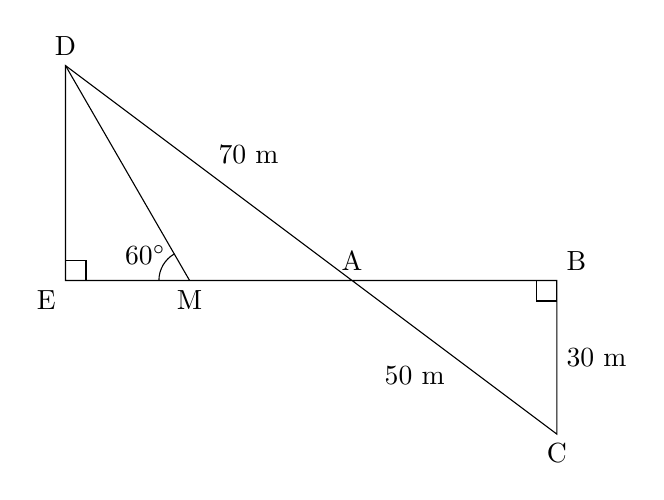
\begin{tikzpicture}[scale=0.65]
            \coordinate[label=above:A](A)at(0,0);
            \coordinate[label=above right:B](B)at(4,0);
            \coordinate[label=below:C](C)at(4,-3);
            \coordinate[label=below:M](M)at(-3.175,0);
            \coordinate[label=below left:E](E)at(-5.6,0);
            \coordinate[label=above:D](D)at(-5.6,4.2);
            \tkzMarkRightAngle[size=0.4](M,E,D)
            \tkzMarkRightAngle[size=0.4](A,B,C)
            \tkzLabelAngle[pos=1](D,M,E){$60^\circ$}
            \tkzMarkAngle[size=0.6](D,M,E)
            \path(D)--(A)node[midway, above right]{70 m};
            \path(A)--(C)node[midway, below left]{50 m};
            \path(B)--(C)node[midway, right]{30 m};
            \draw(E)--(B)--(C)--(D)--cycle;
            \draw(D)--(M);
        \end{tikzpicture}
    \end{center}
    \noindent On a les données suivantes~:
    \begin{itemize}
        \item Les points \mathspoint{A}, \mathspoint{B}, \mathspoint{E} et
        \mathspoint{M}  sont alignés
        \item Les points \mathspoint{A}, \mathspoint{C} et \mathspoint{D} sont
        alignés
        \item \mathspoint{ADE} est un triangle rectangle en \mathspoint{E}
        \item \mathspoint{ABC} est un triangle rectangle en \mathspoint{B}
        \item \mathspoint{AD} = 70 m
        \item \mathspoint{BC} = 30 m
        \item \mathspoint{AC} = 50 m
        \item $\widehat{\mathspoint{DME}}=60^\circ$
    \end{itemize}
    \begin{enumerate}
        \item Calculer la longueur \mathspoint{AB}.
        \item Montrer que les droites \mathspoint{(DE)} et \mathspoint{(BC)}
        sont parallèles.
        \item Montrer que la longueur \mathspoint{DE} est égale à 42 m.
        \item Montrer que la longueur \mathspoint{EM} est environ égale à 24,2 m.
        \item En déduire l'aire du triangle \mathspoint{DEM}.
    \end{enumerate}
    \showthesource
\end{document}